\documentclass{beamer}
\usecolortheme{beaver}
\usepackage{tikz}
\usepackage[utf8]{inputenc}
\usepackage{smartdiagram}
\usepackage{listings}
\usepackage{verbatim}
\usepackage{svg}
\lstset{language=Java,
                basicstyle=\footnotesize\ttfamily,
                keywordstyle=\footnotesize\color{blue}\ttfamily,
}

\usepackage{graphicx}

\title{Git 101}
\author{Víctor Orozco}
\institute{GuateJUG}
\date{\today}

\begin{document}

\frame{\titlepage}

\section{Intro}

\begin{frame}{Víctor Orozco}
     \begin{columns}[T] % contents are top vertically aligned
	     \begin{column}[T]{5cm} % each column can also be its own environment
				\begin{itemize}
				\item Developer (JVM/Open Source Advocate)
				\item Ex-JUG Leader
				\item Consultor independiente (Nabenik)
				\item \href{https://twitter.com/tuxtor}{@tuxtor}
				\item \href{http://vorozco.com}{The J*} 
				\end{itemize}
	     \end{column}
	     \begin{column}[T]{5cm} % alternative top-align that's better for graphics
			\begin{figure}
			\centering
			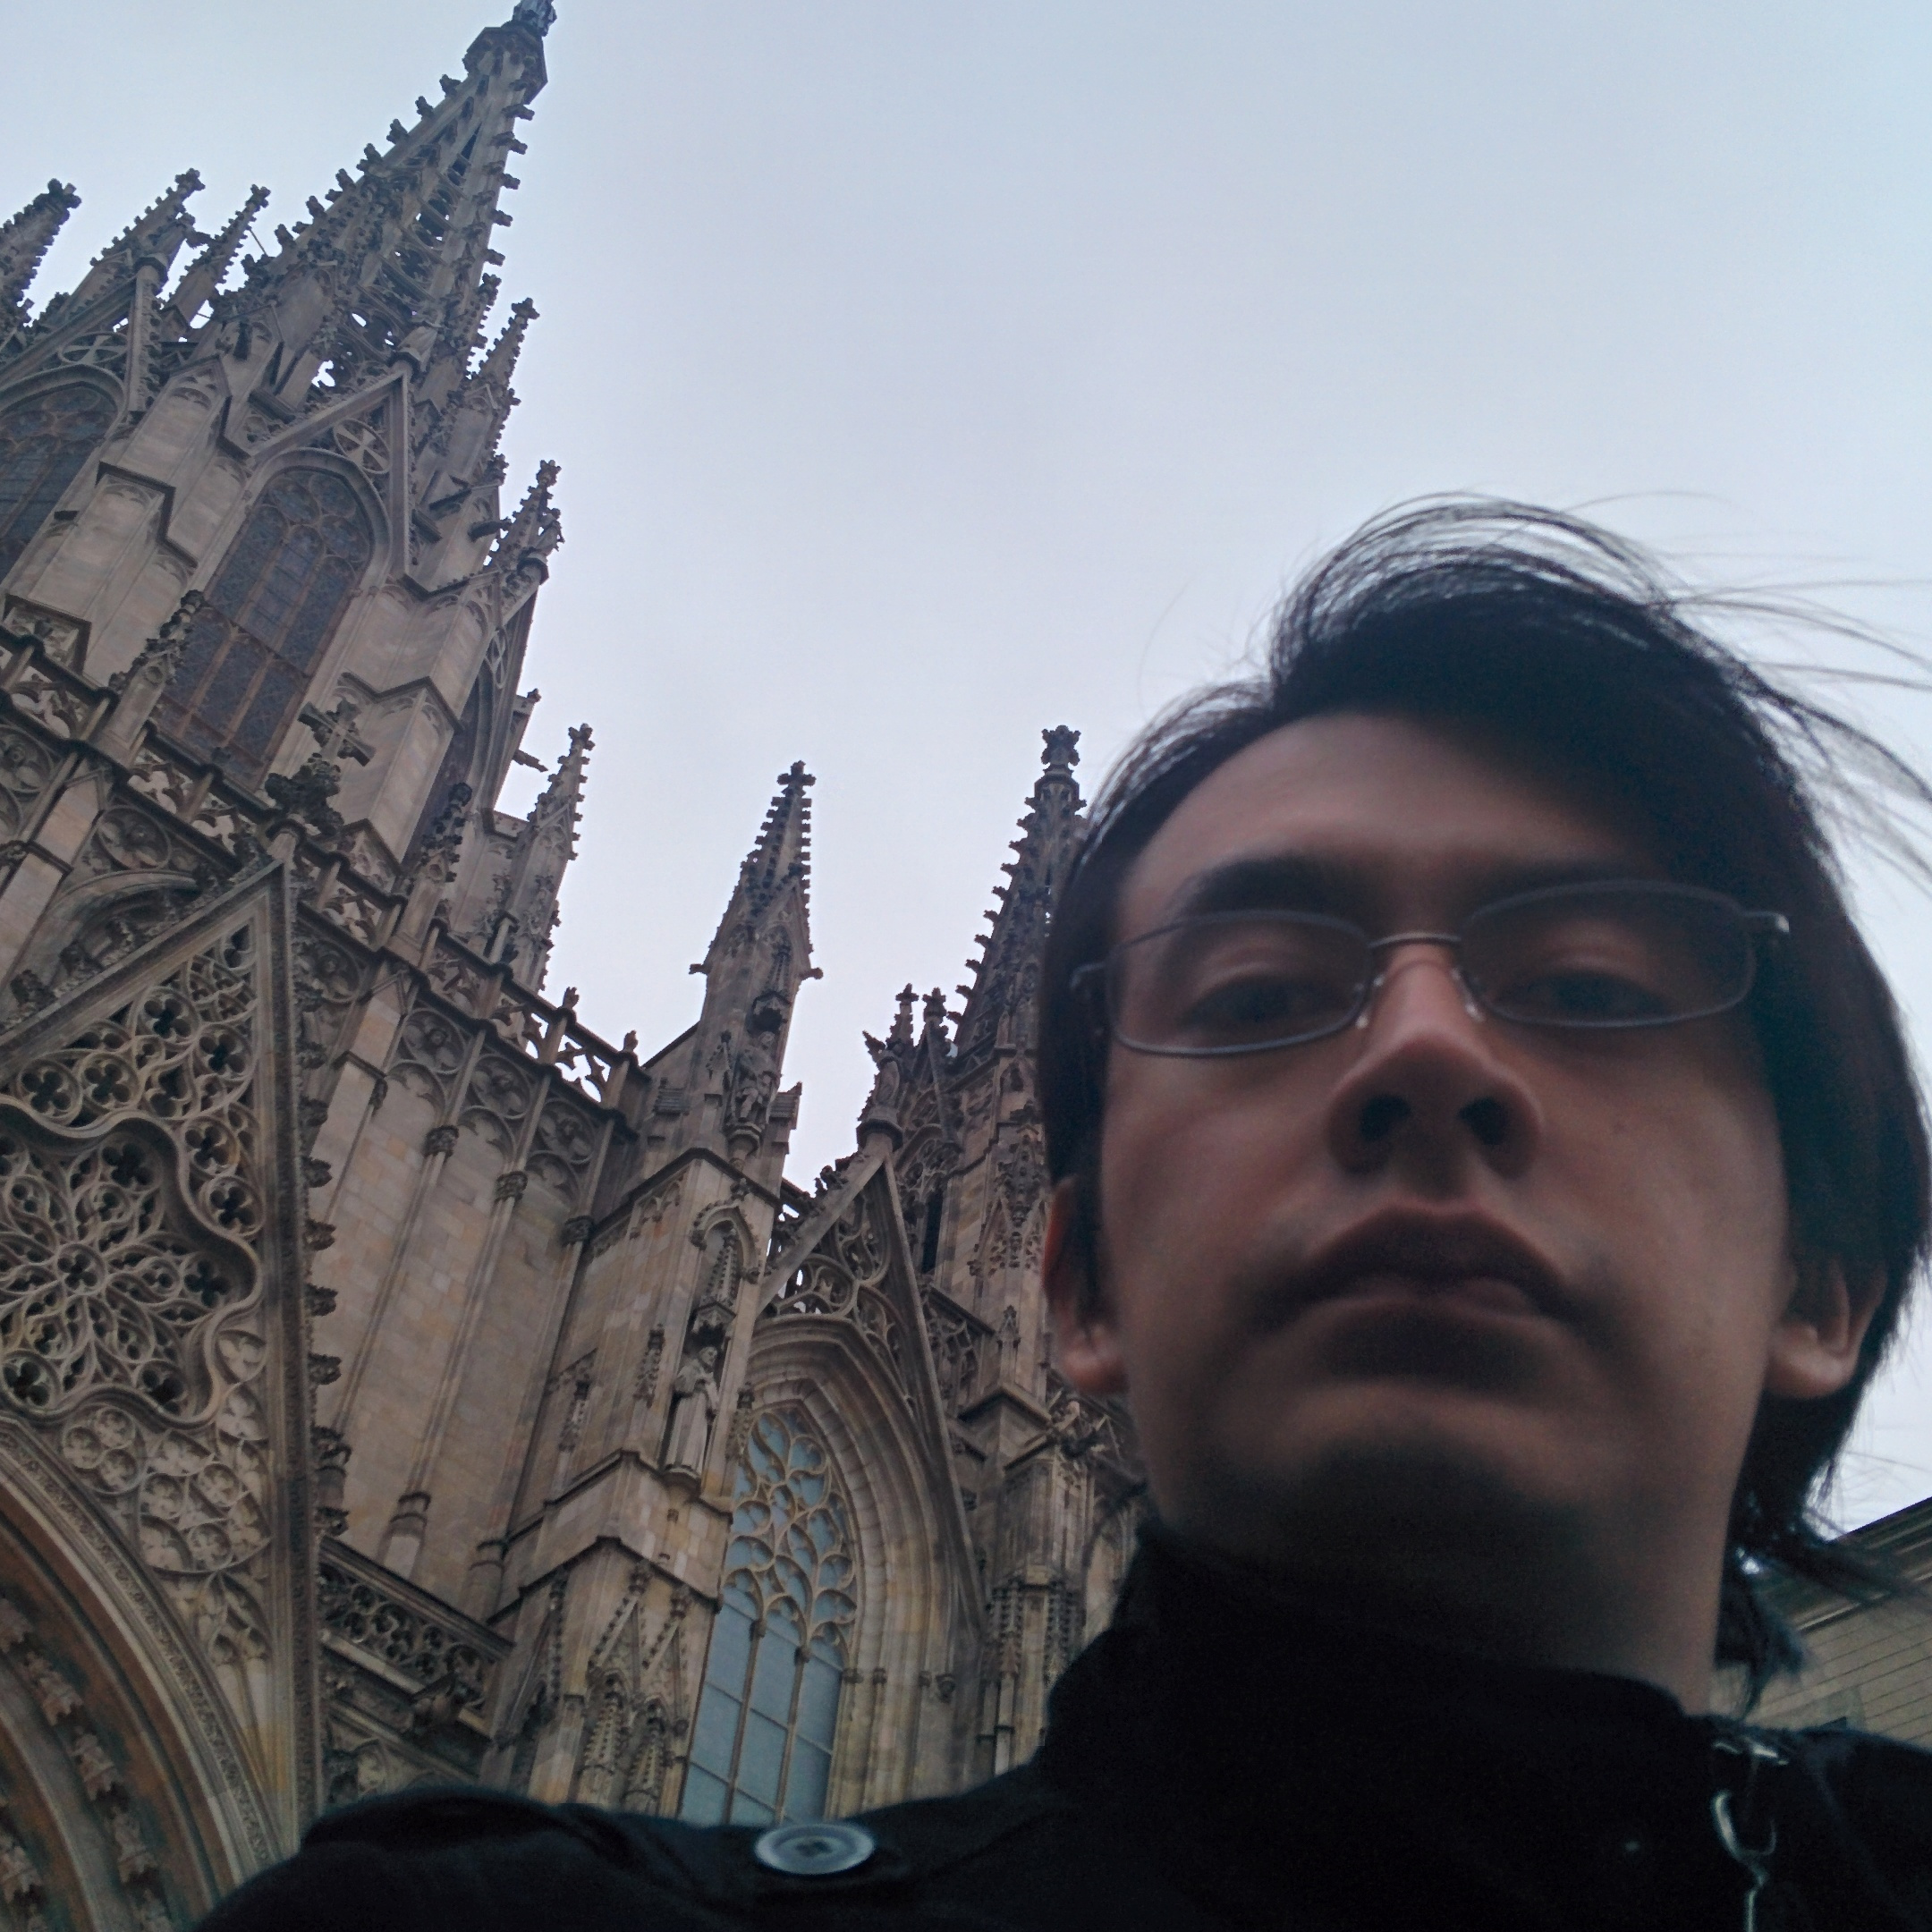
\includegraphics[width=0.7\linewidth]{Images/barcelona.jpg}
			\end{figure}

	     \end{column}
     \end{columns}
\end{frame}

\section{Git Intro}

\begin{frame}{Git (historia)}
	\begin{itemize}
		\item DVCS
		\item Linus Torvalds (2005)
		\item Bitkeeper workflow
		\item "The stupid content tracker
	\end{itemize}
\end{frame}


\begin{frame}{SVN}
\begin{figure}
\centering
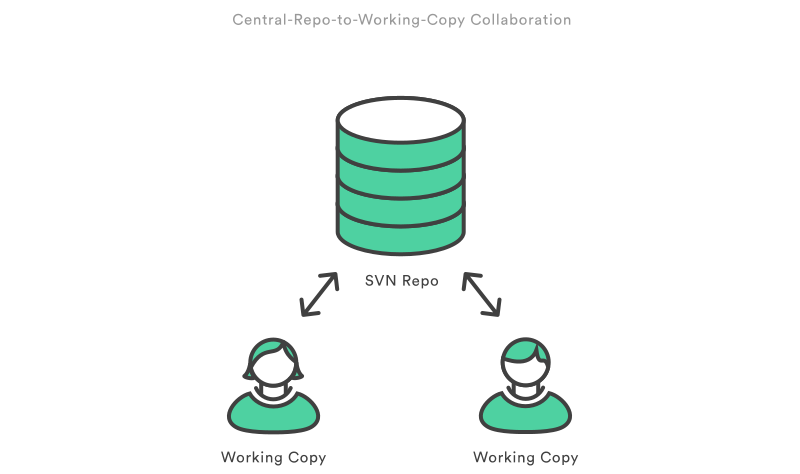
\includegraphics[width=0.7\linewidth]{Images/svn}
\end{figure}
\end{frame}

\begin{frame}{Git}
\begin{figure}
\centering
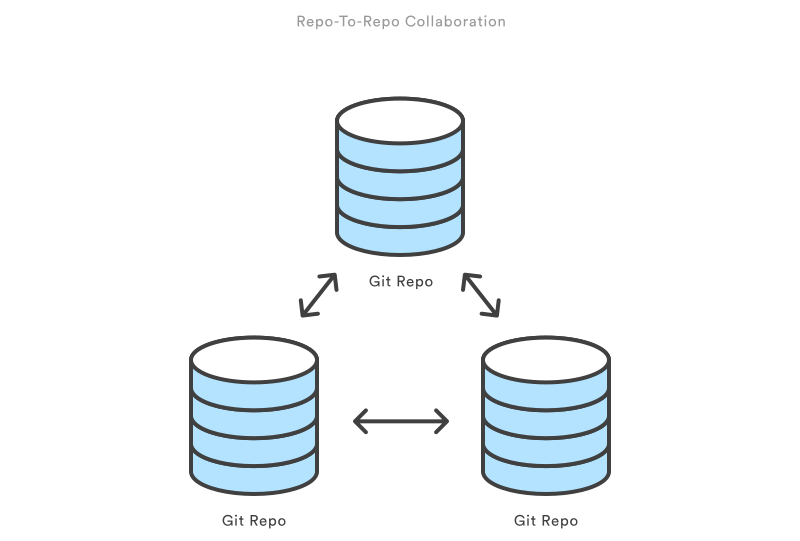
\includegraphics[width=0.7\linewidth]{Images/git}
\end{figure}
\end{frame}



\begin{frame}{Git (caracteristicas)}
	\begin{itemize}
		\item Soporte robusto a metodologias no lineales
		\item Compatibilidad con protocolos estandard (HTTPS, SSH)
		\item Eficiencia con grandes volumenes de datos
		\item Estandard criptografico de nombrado
		\item Modular, toolkit, GPLv2
	\end{itemize}
\end{frame}

\begin{frame}{Git (caracteristicas)}
	\begin{itemize}
		\item Soporte robusto a metodologias no lineales
		\item Compatibilidad con protocolos estandard (HTTPS, SSH)
		\item Eficiencia con grandes volumenes de datos
		\item Estandard criptografico de nombrado
		\item Modular, toolkit, GPLv2
	\end{itemize}
\end{frame}

\section{Git primeros pasos}
\begin{frame}{Git}
	Setup
\end{frame}

\begin{frame}[fragile]{Git workflow}
	Creamos un repositorio
	\begin{verbatim}
		git init
	\end{verbatim}
\end{frame}

\begin{frame}[fragile]{Git workflow}
	Copiamos un repositorio local
	\begin{verbatim}
		git checkout /path/to/repository
	\end{verbatim}
	
	Copiamos un repositorio remoto
	\begin{verbatim}
		git checkout username@host:/path/to/repository
	\end{verbatim}
\end{frame}

\begin{frame}[fragile]{Git workflow}
	Consiste en tres arboles
	\begin{itemize}
	\item Working directory
	\item Staging
	\item HEAD
	\end{itemize}
	\begin{figure}
		\centering
		
\includegraphics[width=0.7\linewidth]{Images/trees}
	\end{figure}
\end{frame}

\begin{frame}[fragile]{Git workflow}
	Ejemplo add \& commit
	\begin{verbatim}
		git add <filename>
		git commit -m "Creando mi primer archivo git"
	\end{verbatim}	
\end{frame}

\begin{frame}[fragile]{Git config}
	\begin{verbatim}
		git config --global user.name <name>
		git config --global user.email <email>
	\end{verbatim}	
\end{frame}


\begin{frame}[fragile]{Git workflow}
	Enviar a servidor remoto
	\begin{itemize}
	\item git push $<$remote$>$ $<$branch$>$
	\item git remote add $<$remote$>$ $<$url$>$
	\end{itemize}
	\begin{verbatim}
		git remote add origin <server<
		git push origin master
	\end{verbatim}
\end{frame}


\begin{frame}[fragile]{Git branching}	
	\begin{itemize}
	\item Isolar caracteristicas entre si
	\item \textbf{master} es la rama predefinida
	\end{itemize}
	\begin{verbatim}
			git checkout -b <branch>
			git push origin <branch>
	\end{verbatim}
	\begin{figure}
			\centering
			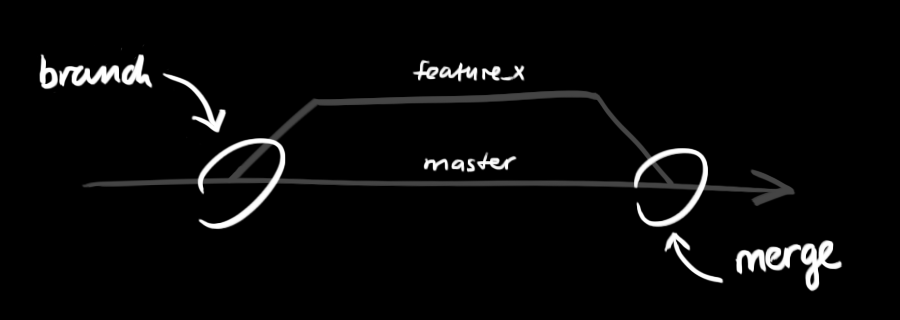
\includegraphics[width=0.7\linewidth]{Images/branches}
	\end{figure}
\end{frame}


\begin{frame}[fragile]{Git merge}	
	\begin{itemize}
	\item Integrar caracteristicas desde una rama
	\item Rama actual = rama donde se integrara el cambio
	\end{itemize}
	\begin{verbatim}
			git checkout master
			git merge <branch>
			git branch -d <branch>
	\end{verbatim}
\end{frame}

\begin{frame}[fragile]{Git update}	
	\begin{verbatim}
			git pull //obtiene cambios remotos
			git merge <branch>
	\end{verbatim}
\end{frame}

\begin{frame}[fragile]{Git log}	
	\begin{verbatim}
			git log
			git log --pretty=oneline
			git log --graph --oneline --decorate --all
			git log --name-status //archivos cambiados
	\end{verbatim}
\end{frame}

\begin{frame}[fragile]{Git tagging}	
	\begin{verbatim}
			 git tag 1.0.0 1b2e1d63ff
	\end{verbatim}
\end{frame}

\begin{frame}[fragile]{Git replace}	
	\begin{verbatim}
			 git checkout -- <filename>
	\end{verbatim}
	Obtiene el ultimo HEAD, cambios en index y new file son conservados
\end{frame}

\section{Git advanced workflows}

\begin{frame}{Workflows}
	\begin{itemize}
		\item Centralized
		\item Feature branch
		\item \textbf{Gitflow}
		\item \textbf{Forking}
	\end{itemize}
\end{frame}


\begin{frame}{Centralized}
\begin{figure}
\centering
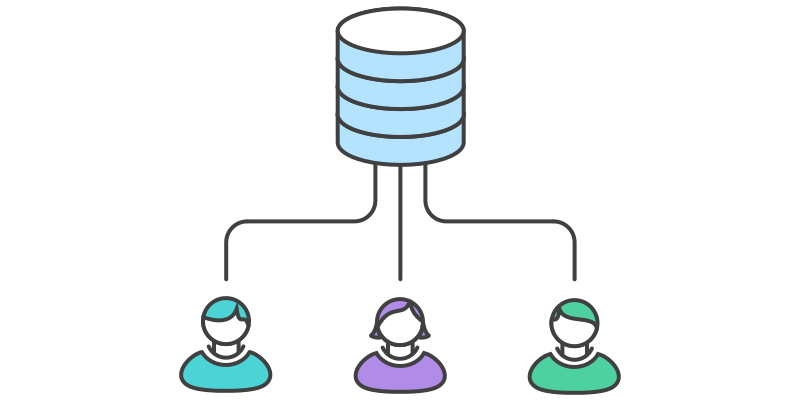
\includegraphics[width=0.7\linewidth]{Images/centralized}
\end{figure}
\end{frame}

\begin{frame}{Feature branch}
\begin{figure}
\centering
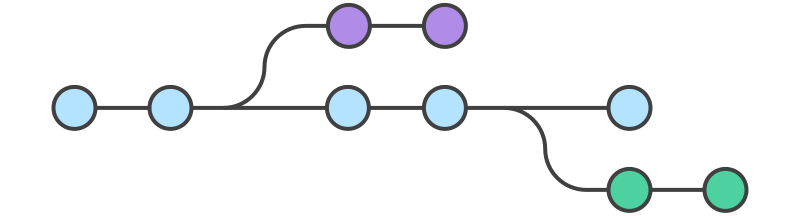
\includegraphics[width=0.7\linewidth]{Images/feature.png}
\end{figure}
\end{frame}

\begin{frame}{Gitflow}
\begin{figure}
\centering
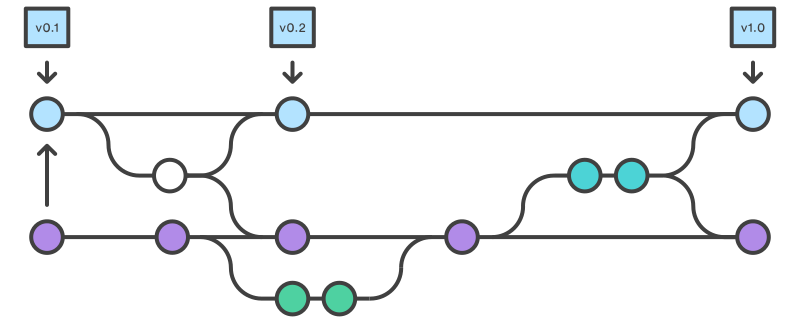
\includegraphics[width=0.7\linewidth]{Images/gitflow.png}
\end{figure}
\end{frame}

\begin{frame}{Forking}
\begin{figure}
\centering
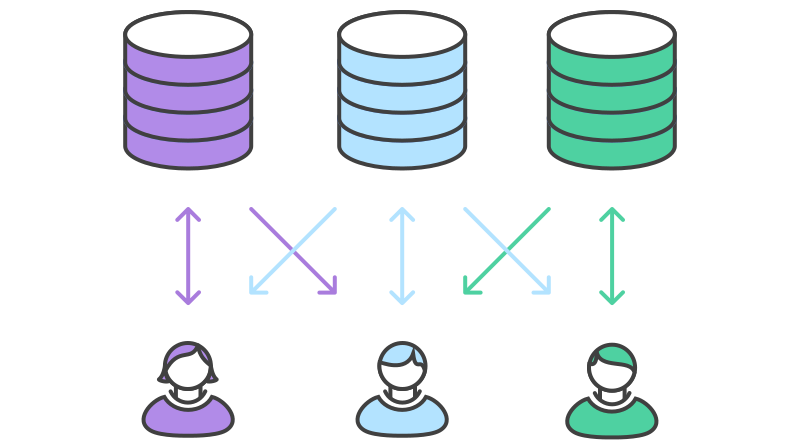
\includegraphics[width=0.7\linewidth]{Images/forking.png}
\end{figure}
\end{frame}

\begin{frame}{Recursos}
\begin{itemize}
\item \href{https://www.atlassian.com/git/tutorials}{Atlassian Git Tutorials}
\item \href{https://try.github.io/levels/1/challenges/1}{Git School}
\end{itemize}

\end{frame}



\begin{frame}{Gracias}
\begin{itemize}
\item me@vorozco.com
\item http://vorozco.com
\item http://github.com/tuxtor/slides
\end{itemize}
\begin{center}

\includegraphics[width=0.1\linewidth]{Images/cclogo}
\\
This work is licensed under a Creative Commons Attribution-ShareAlike 3.0 Guatemala License.
\end{center}
\end{frame}
\end{document}

